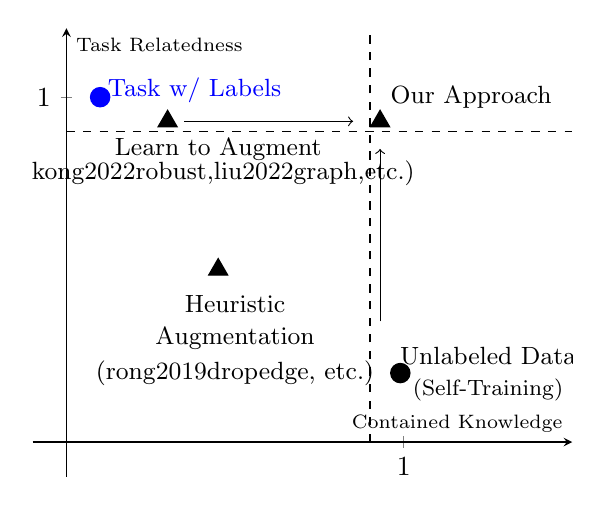
\begin{tikzpicture}
    \begin{axis}
    [
        legend pos= north east,
        axis lines = center,
        domain=-1:2,
        xlabel={\scriptsize Contained Knowledge},
        xmin=-0.1,
        xmax=1.5,
        xtick={0, 1},
        ylabel={\scriptsize Task Relatedness},
        ymin=-0.1,
        ytick={0, 1},
        ymax=1.2,
    ]
    % purple pentagon
    \addplot[only marks, color=black, mark=triangle*, mark size=4pt] coordinates { (0.93,0.93) };
    \node[] at (axis cs: 1.2, 1.0) {\textcolor{black}{\small Our Approach}};

    
    % magenta
    \addplot[only marks, color=black, mark=triangle*,mark size=4pt] coordinates {(0.3,0.93)};
    \node[] at (axis cs: 0.45,0.85) {\textcolor{black}{\small Learn to Augment}};
    \node[] at (axis cs: 0.45,0.78) {\small (\citeauthor{kong2022robust},\citeauthor{liu2022graph},etc.)};
    
    % cyan
    \addplot[only marks, color=black, mark=triangle*,mark size=4pt]
        coordinates {(0.45,0.5) };
    \node[] at (axis cs: 0.5,0.4) {\textcolor{black}{\small Heuristic}};
    \node[] at (axis cs: 0.5,0.3) {\textcolor{black}{\small Augmentation}};
    \node[] at (axis cs: 0.5,0.2) {\textcolor{black}{\small (\citeauthor{rong2019dropedge}, etc.)}};
    
    % red square
    \addplot[only marks, color=blue, mark=*, mark size=3.5pt]
        coordinates {(0.1,1)};
    \node[] at (axis cs: 0.38,1.02) {\textcolor{blue}{\small Task w/ Labels}};

    % color=blue
    \addplot[only marks, color=black, mark=*, mark size=3.5pt]
        coordinates {(0.99,0.2) };
    \node[] at (axis cs: 1.25,0.25) {\textcolor{black}{\small Unlabeled Data}};
    \node[] at (axis cs: 1.25,0.15) {\textcolor{black}{\footnotesize (Self-Training)}};
    
    \draw [dashed] (0.9,0) -- (0.9,1.2);
    \draw [dashed] (0,0.9) -- (1.5,0.9);
    \draw[->](axis cs: 0.35,0.93)--(axis cs: 0.85,0.93);
    \draw[->](axis cs: 0.93,0.35)--(axis cs: 0.93,0.85);
    % \draw[->](unlabeled)--(ours);
    \end{axis}
\end{tikzpicture}